% Para cuando se tenga la carta firmada, scaneada y en formato PDF
% 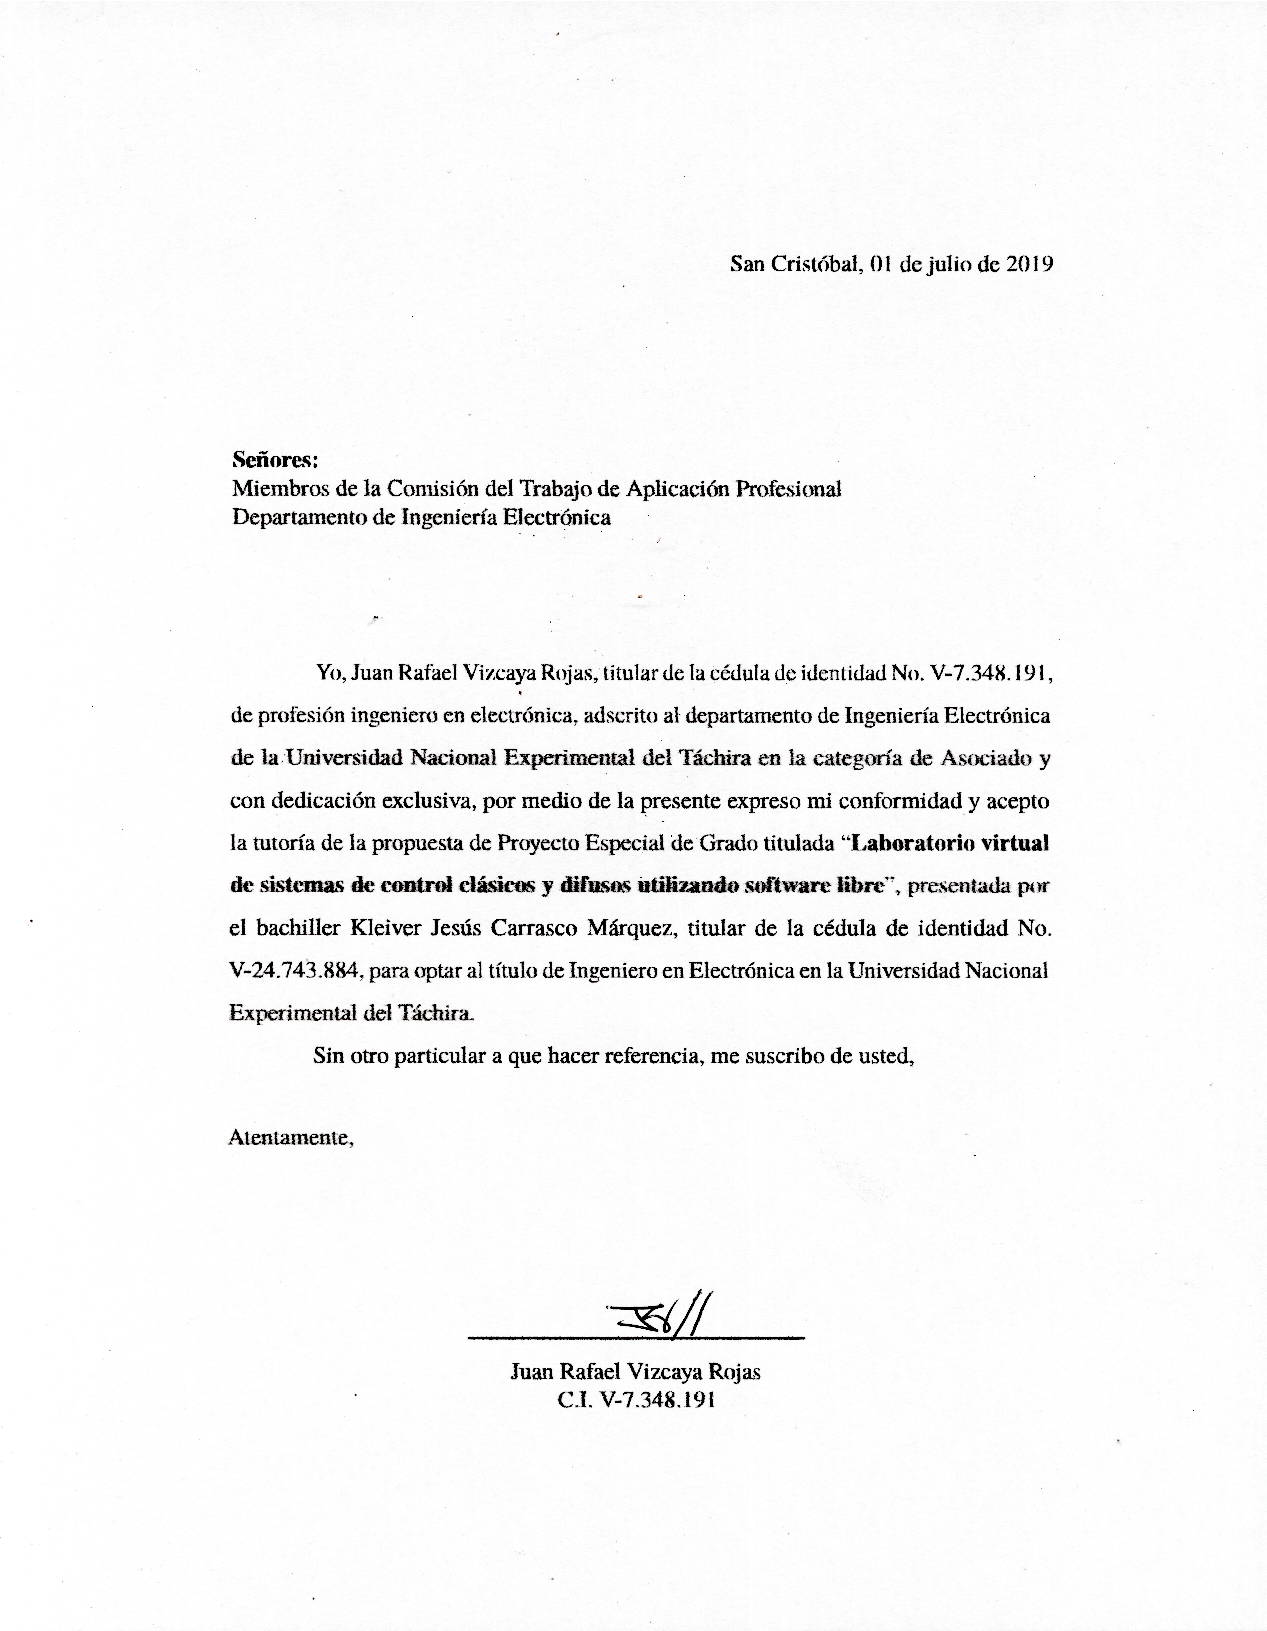
\includepdf[pages=-, fitpaper, templatesize={\paperwidth}{\paperheight},
% 			pagecommand={\thispagestyle{empty}\setcounter{page}{3}}
% 			]{carta_aceptacion}

% Generacion de la carta
\begin{titlepage}
\parskip=7.25pt plus 2pt
\setcounter{page}{3}
\begin{flushright}
	San Cristóbal, \today
\end{flushright}

\vspace{1cm}
\vfill

\begin{flushleft}
		\singlespacing
		
		\setlength{\parskip}{0pt}
		
		\textbf{Señores:}
		
		Miembros de la Comisión del Trabajo de Aplicación Profesional
		
		Departamento de Ingeniería Electrónica
		
\end{flushleft}

\vfill
\begin{spacing}{1.5}
	Yo, Juan Rafael Vizcaya Rojas, titular de la cédula de identidad No. \mbox{V-7.348.191}, de profesión ingeniero en electrónica, adscrito al departamento de Ingeniería Electrónica de la Universidad Nacional Experimental del Táchira en la categoría de Asociado y con dedicación exclusiva, por medio de la presente expreso mi conformidad y acepto la tutoría de la propuesta de Proyecto Especial de Grado titulada \enquote{\textbf{Laboratorio virtual de sistemas de control clásicos y difusos utilizando software libre}}, presentada por el bachiller Kleiver Jesús Carrasco Márquez, titular de la cédula de identidad No. \mbox{V-24.743.884}, para optar al título de Ingeniero en Electrónica en la Universidad Nacional Experimental del Táchira.
	
	Sin otro particular a que hacer referencia, me suscribo de usted,
	
	\setlength{\parskip}{20pt} 
	
	\noindent Atentamente,
\end{spacing}

\vfill

\begin{center}
	
	\rule{6cm}{1pt}
	
	\vspace{0.2cm}
	
	\parskip=0pt plus 2pt
    
    \begin{spacing}{1}    
        Juan Rafael Vizcaya Rojas
    
        C.I. V-7.348.191
    \end{spacing}
\end{center}

\vspace{0.5cm}

\end{titlepage}